%%==================================================================%%
%% Author : Tejedo Gonz�lez, Daniel                                 %%
%%          S�nchez Barreiro, Pablo                                 %%
%% Version: 1.0, 25/11/2012                                         %%                   %%                                                                  %%
%% Memoria del Proyecto Fin de Carrera                              %%
%% Sintaxis abstracta,  pruebas                                       %%
%%==================================================================%%

Las pruebas en este punto del dise�o no fueron especialmente fruct�feras, ya que la creaci�n de la gram�tica para la sintaxis textual de nuestro lenguaje motiv� numerosos cambios en un metamodelo que en este punto parec�a totalmente correcto. Las pruebas consistieron en la creaci�n de varias instancias del metamodelo y observar su �rbol de creaci�n, comprobando si este se correspond�a con el de diversas instrucciones que fuimos creando intentando tener en cuenta todos los casos. 

No fueron especialmente rigurosas dado que a estas alturas del desarrollo de la aplicaci�n a�n falta muchos elementos implicados por crear que sin duda tendr�an repercusi�n en nuestra sintaxis abstracta, como de hecho ocurri� m�s adelante. 

\begin{figure}[t]
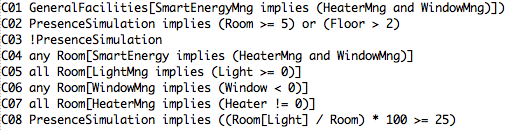
\includegraphics[scale=0.6]{metamodelo/instpruebas.jpg}
\caption{Conjunto de instrucciones que puso a prueba el funcionamiento}
\label{figmetains}
\end{figure}

Las instrucciones que fueron puestas a prueba, y que se comprob� que en efecto eran parseadas de un modo apropiado, fueron las que se ven en la figura \ref{figmetains}. Este conjunto de instrucciones servir�n como pruebas tambi�n en momentos m�s avanzados del desarrollo.